\chapter{Model}\label{chap:Model}
A description of the physical behavior of the quadcopter is convenient in order to achieve a steady flight. From the obtained model, a control system can be designed such that the desired flying characteristics are obtained.

In this chapter, an overview is first presented. Then, the model is derived and a linear approximation is performed. Finally, these two are compared in simulation. This ensures that the linear approximation yields acceptable results.

\section{Model Overview} \label{sec:ModelOverview}
The model can be split into two submodels, one describing the angular behaviour and the other being a translational model.
\begin{figure}[H]
    \centering
    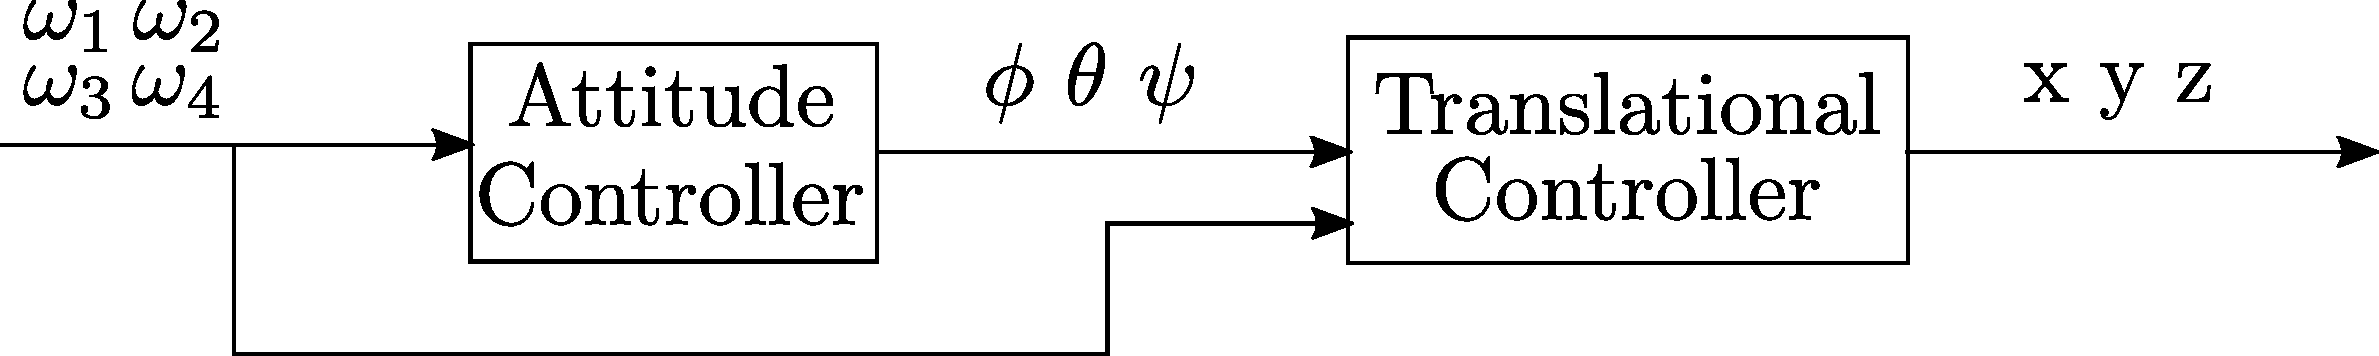
\includegraphics[scale=0.3]{figures/modelOverview}
    \caption{Overview of how the two models are related.}
    \label{fig:modelOverview}
\end{figure}
%
\autoref{fig:modelOverview} shows the relation between the two submodels. The attitude model, that the describes the angular behaviour, get the velocities of the four motors as input its output is the angles pitch, roll and yaw. These angles are input of the translational model. The translational model do also have the velocities of the motors as input, resulting in seven inputs in total. The output of the translational model is a position given in the x, y and z axes.

Another consideration to be made before modeling the quadcopter is the usage of two coordinate frames. A body frame, that is fixed to the flying object and an inertial frame, that is fixed to the Vicon room. 
%
\begin{figure}[H]
    \centering
    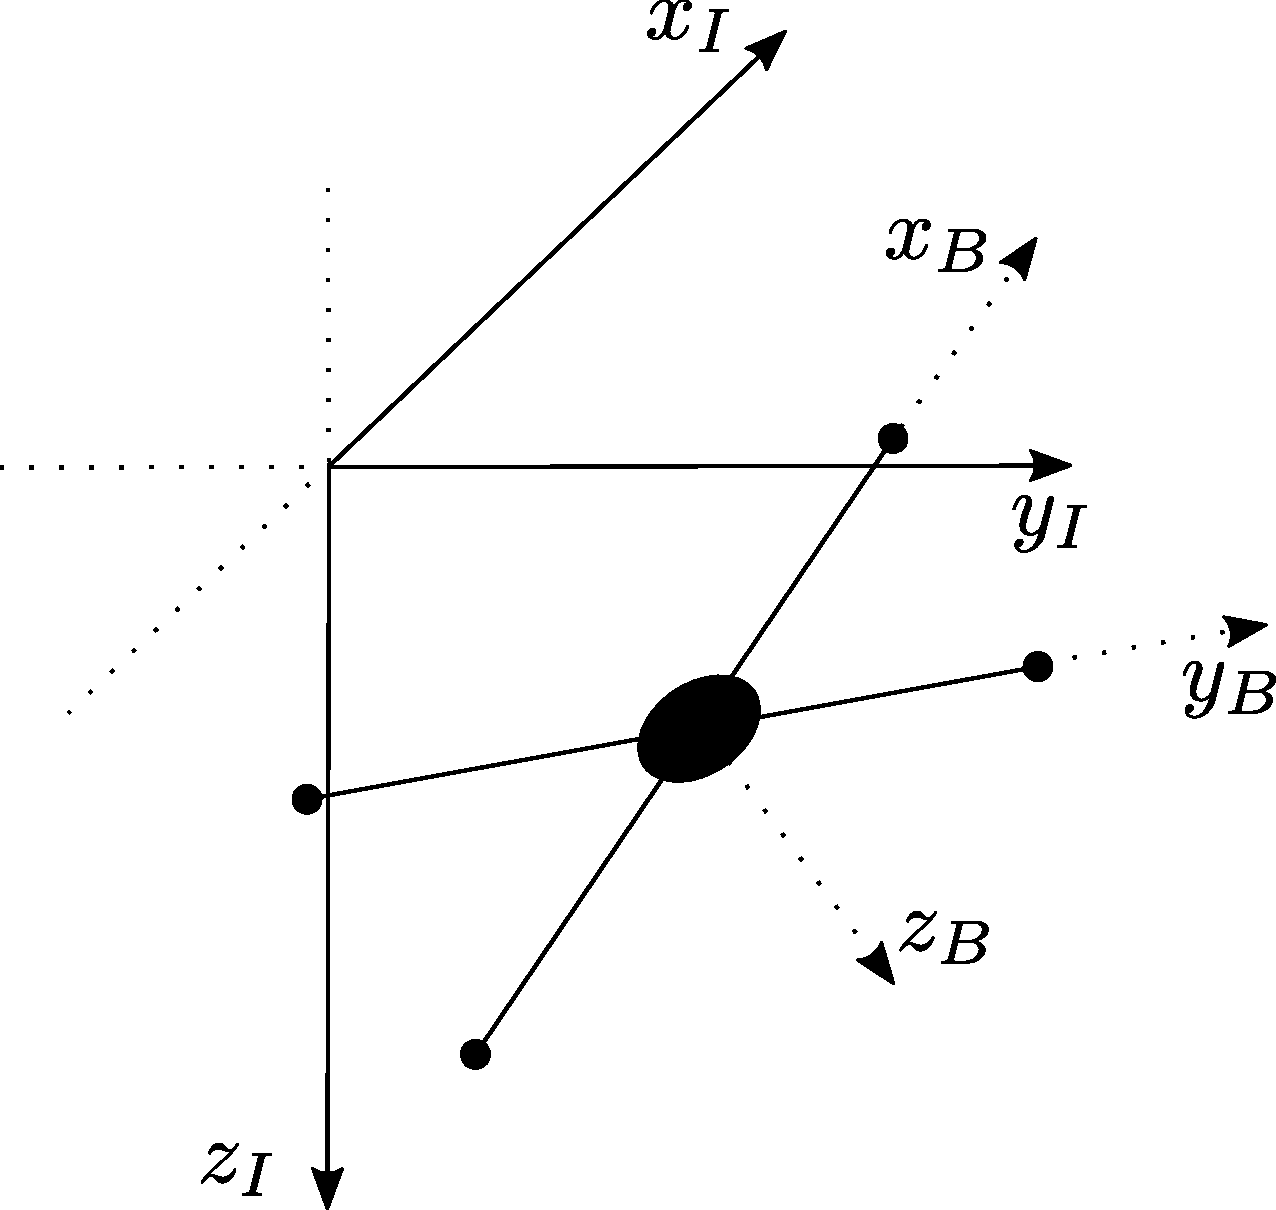
\includegraphics[scale=0.25]{figures/framesDiagram}
    \caption{The quadcopter with its body frame (B-index) placed in the intial frame (I-index) of the Vicon room. }
    \label{fig:framesDiagram}
\end{figure}

\autoref{fig:framesDiagram} shows the two frames, which are necessary to use, as it is desired to know where the quadcopter is within the inertial frame to determine its position. To obtain the orientation of the quadcopter, the body frame's orientation is compared to the inertial frame and yields the angles of roll, pitch and yaw. 

The transformation from the body frame to the inertial one is done through a  rotation matrix, \autoref{eq:RotMatrix}, that describes a total rotation in terms of three consecutive rotations, assuming first in roll, then in pitch and finally in yaw.
%
\footnotesize
\begin{flalign}
	\si{R_{\phi, \theta, \psi}} &=
	\begin{bmatrix}
		\ \si{c(\theta) \cdot c(\psi)}                & \si{-c(\theta) \cdot s(\psi)}  & \si{-c(\phi) \cdot s(\theta) \cdot c(\psi) + s(\phi) \cdot s(\psi)}  \ \ \ \\ 
		\ \si{s(\phi) \cdot s(\theta) \cdot s(\psi) + c(\phi) \cdot s(\psi)}  	  & \si{-s(\phi) \cdot s(\theta) \cdot s(\psi) + c(\phi) \cdot c(\psi)} 		& \si{c(\phi) \cdot s(\theta) \cdot s(\psi) + s(\phi) \cdot c(\psi)}                \ \ \ \\ 
		\ \si{s(\theta)}      	  & \si{-s(\phi) \cdot c(\theta)}    		& \si{c(\phi) \cdot c(\theta)}                 \ \ \ 
	\end{bmatrix} 	\label{eq:RotMatrix}
\end{flalign}
\normalsize
%
\begin{where}
\va{R_{\phi, \theta, \psi}}{is the rotation matrix}{}
\va{\phi}{is the roll}{rad}
\va{\theta}{is the pitch}{rad}
\va{\psi}{is the yaw}{rad}
\end{where}

It shall be noted, that due to the size of the matrix sine and cosine are referenced $s$ and $c$ respectively.

Once these considerations have been taken into account, the two submodels can be derived.
 
%Angle and Linear
%Explain the two frames and include drawing showing them
%Flow of the chapter

%\Figref{diagramQuad} shows a representation of the quadcopter where two reference systems, inertial and body, can be seen, as well as the conventions for angles of rotation and forces. \Figref{diagramTorque} shows the body from above and includes the chosen convention for the torques produced by the propellers.
%
%\begin{minipage}{\linewidth}
%	\begin{minipage}{0.45\linewidth}
%		\begin{figure}[H]
%			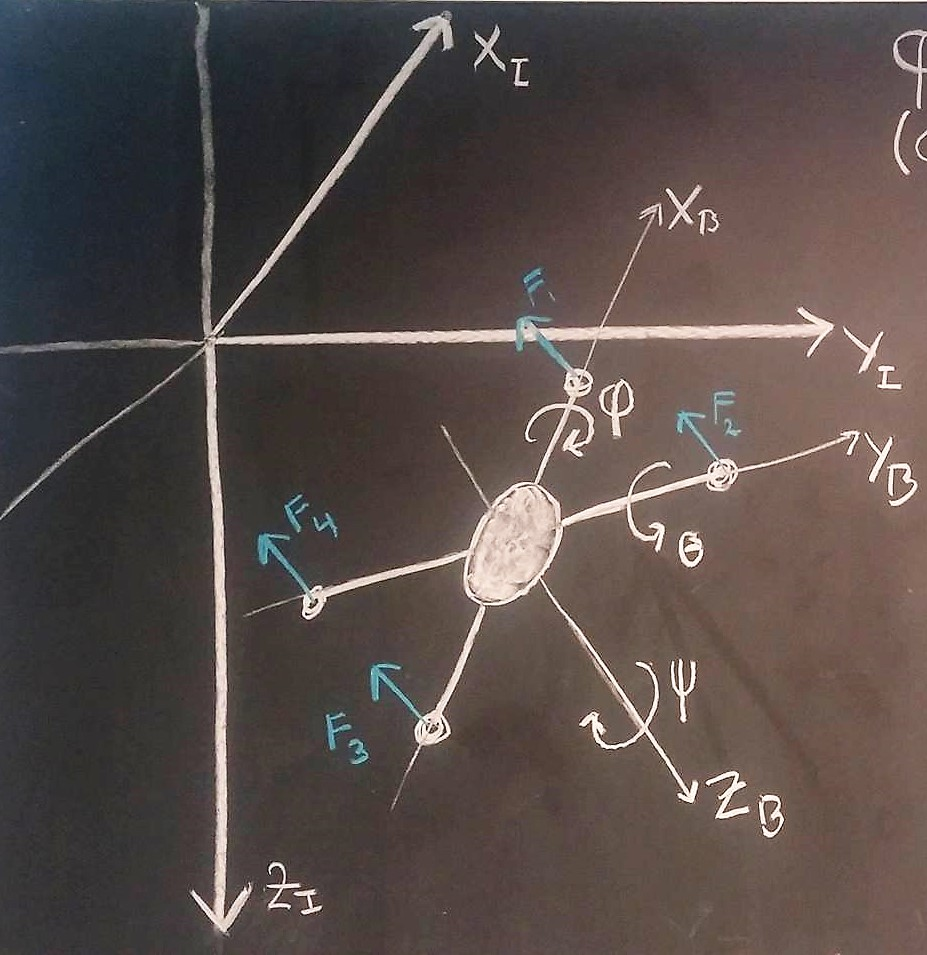
\includegraphics[scale=.27]{figures/drone_diagram}
%			\centering
%			\captionsetup{justification=centering}
%			\captionof{figure}{Diagram of the quadcopter which includes inertial and body reference systems, as well as the references for the angles (roll, pitch and yaw) and the thrust forces produced by the propeller. }
%			\label{diagramQuad}
%		\end{figure}
%	\end{minipage}
%	\hspace{0.03\linewidth}
%	\begin{minipage}{0.45\linewidth}
%		\begin{figure}[H] \vspace{16mm}
%			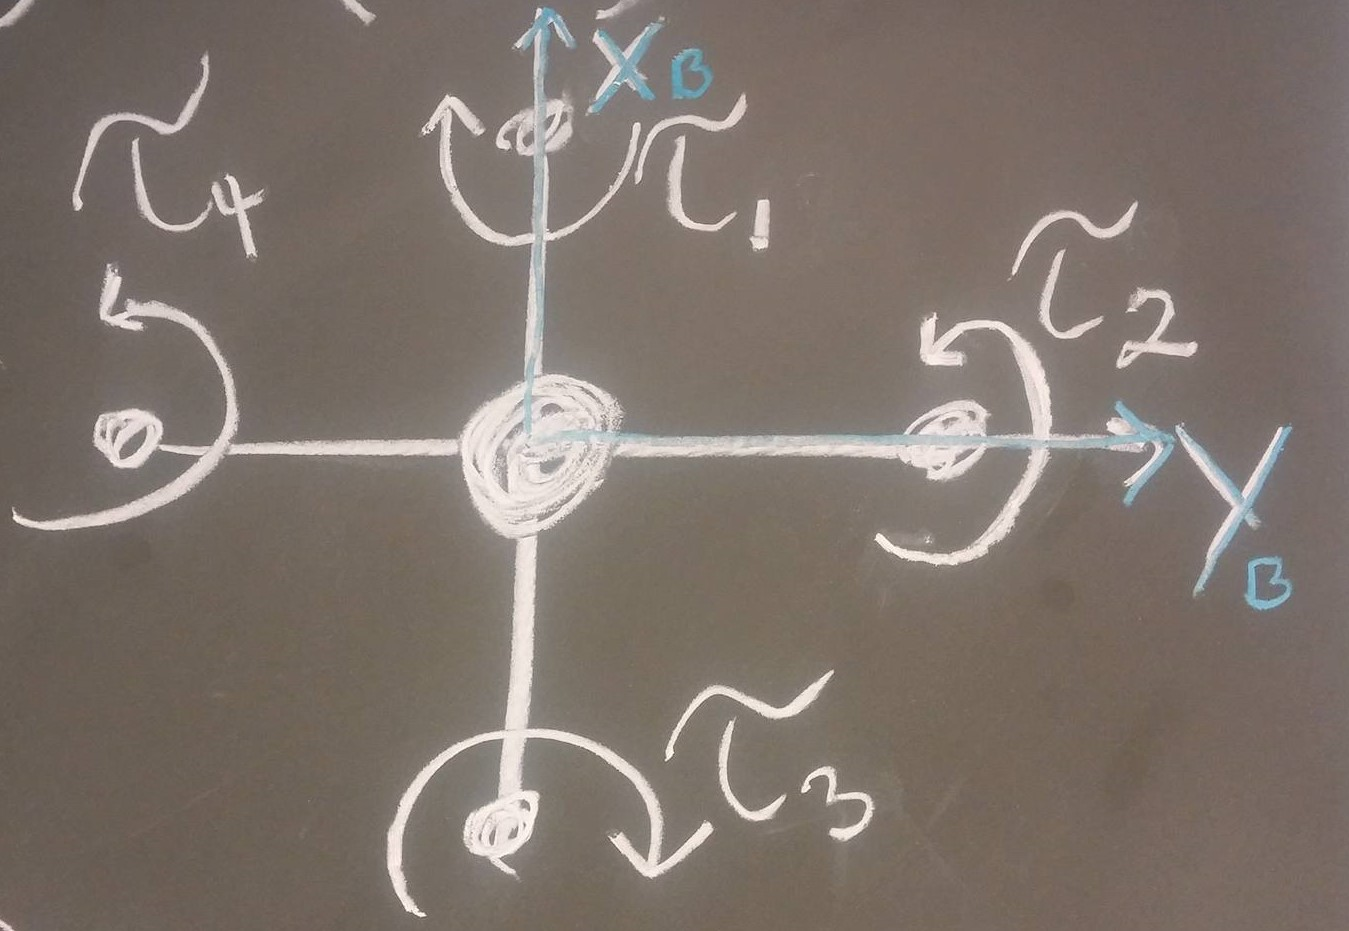
\includegraphics[scale=.18]{figures/torques_diagram}
%			\centering
%			\captionsetup{justification=centering}
%			\captionof{figure}{Diagram of the quadcopter from above, with the references for the torques produced by the drag force at the propeller.}
%			\label{diagramTorque}
%		\end{figure}
%	\end{minipage}
%\end{minipage}
%In the following section the attitude model is derived. 